\documentclass[review]{elsarticle}

\usepackage{lineno,hyperref}
\usepackage{tikz, pgf, graphicx}
\usetikzlibrary{shapes.geometric, arrows,positioning,matrix,calc,intersections}
\modulolinenumbers[5]

\journal{Journal of \LaTeX\ Templates}

%%%%%%%%%%%%%%%%%%%%%%%
%% Elsevier bibliography styles
%%%%%%%%%%%%%%%%%%%%%%%
%% To change the style, put a % in front of the second line of the current style and
%% remove the % from the second line of the style you would like to use.
%%%%%%%%%%%%%%%%%%%%%%%

%% Numbered
%\bibliographystyle{model1-num-names}

%% Numbered without titles
%\bibliographystyle{model1a-num-names}

%% Harvard
%\bibliographystyle{model2-names.bst}\biboptions{authoryear}

%% Vancouver numbered
%\usepackage{numcompress}\bibliographystyle{model3-num-names}

%% Vancouver name/year
%\usepackage{numcompress}\bibliographystyle{model4-names}\biboptions{authoryear}

%% APA style
%\bibliographystyle{model5-names}\biboptions{authoryear}

%% AMA style
%\usepackage{numcompress}\bibliographystyle{model6-num-names}

%% `Elsevier LaTeX' style
\bibliographystyle{elsarticle-num}
%%%%%%%%%%%%%%%%%%%%%%%

\begin{document}

\begin{frontmatter}

\title{Elsevier \LaTeX\ template\tnoteref{mytitlenote}}
\tnotetext[mytitlenote]{Fully documented templates are available in the elsarticle package on \href{http://www.ctan.org/tex-archive/macros/latex/contrib/elsarticle}{CTAN}.}

%% Group authors per affiliation:
\author{Elsevier\fnref{myfootnote}}
\address{Radarweg 29, Amsterdam}
\fntext[myfootnote]{Since 1880.}

%% or include affiliations in footnotes:
\author[mymainaddress,mysecondaryaddress]{Elsevier Inc}
\ead[url]{www.elsevier.com}

\author[mysecondaryaddress]{Global Customer Service\corref{mycorrespondingauthor}}
\cortext[mycorrespondingauthor]{Corresponding author}
\ead{support@elsevier.com}

\address[mymainaddress]{1600 John F Kennedy Boulevard, Philadelphia}
\address[mysecondaryaddress]{360 Park Avenue South, New York}

\begin{abstract}
This template helps you to create a properly formatted \LaTeX\ manuscript.
\end{abstract}

\begin{keyword}
\texttt{elsarticle.cls}\sep \LaTeX\sep Elsevier \sep template
\MSC[2010] 00-01\sep  99-00
\end{keyword}

\end{frontmatter}




\linenumbers

\section{Introduction}
Composite materials offer improved strength, stiffness, corrosion resistance, etc. over conventional
materials, and are widely used as alternative materials for applications in various industries
ranging from electronic packaging to golf clubs, and medical equipment to homebuilding, making
aircraft structure to space vechicles. One widely known advange of using composite material is can
significantly reducing the weight of target structure.  


thickness\cite { schmit1973optimum, schmit1977optimum, fukunaga1991strength, soares1995discrete,
	le1995improved, jayatheertha1996application, wang1996optimum, adali1997minimum,
	correia1997higher, scares1997optimization, abu1998optimum, lombardi1998anti, le1998design,
	sivakumar1998optimum, barakat1999use, richard2000reliability, moita2000sensitivity,
soremekun2001composite, walker2003technique, di2003multiconstrained, kere2003using}



Genetic
algorithm(GA)\cite{callahan1992optimum,soremekun2001composite,park2001stacking,walker2003technique,deka2005multiobjective,pelletier2006multi,jadhav2007parametric,kim2007development,park2008improved,}

Colony Optimization\cite{aymerich2006ant,}



In practice, fiber orientations are restricted to a finite set of angles, and ply thickness is a
specific numberic value.  Because the design variables are not continueous, a gradient based
optimization procedure, such as gradient descent method, is not suitable to cope with such problems.
Moreover, gradient based optimization approach is very eazily to get trapped in local minima, and
many local optimum may exist in structural optimization problems. A stochastic optimization, such as
genetic algorithm(GA) and simulated annealing(SA), is able to deal with optimization problem with
discrete variables. Besides, stochastic method could escape from local optimum, and obtain global
optimum.  GA is one of the most reliably stochastic algorithm, which has been widely used in solving
constraint desgin for composite laminate. Although GA gains different advantages for solving
discrete problems, many disadvantages exists within this approach. First, the optimization process
of GA parameters, such as the population size, parent population,mutation percentage, etc., is very
tedious; Second, the GA needs to evaluate the objective functions many times to acheive the
optimization, and the compuation cost is very high; the last problem within GA is the premature
convergence. GA consists of five basic parts: the variable coding, selection scheme, crossover
operator, mutation operator and how the constraints are handled.

The first issue when implementing a GA is the representation of design variables, because an
appropriate design representation is crucial to enhance the efficiency of GA. Real value string has
been widely employed in 

Selection scheme plays a critical role in balancing the dilemma of exploration and exploitation
inherented in GA, and various selection methods, for example, roulette wheel, elitist, and tournament
etc., have been proposed to overcome this issue. Both of roulette selection and tournament selection
are well-studied and widely employed in the optimization design of laminated composite due to their
simplicity to code and efficiency for both nonparallel and parallel architectures.


multiple types of crossover operator has been utilized in the optimization design of composite
structures, such as: one-point, two-point, and uniform crossover.



GA is originally proposed for unconstrained optimization. However, in order to deal with constrained
design for composite laminate, some techiques were introduced into the GA. The first method is using
of data structure, special data structure was developed to fulfils the symmetry constraint of the
laminate, which consists of coding only half of the laminate and considering that each stack of the
laminate is formed by two laminae with the same orientation but opposite
signs\cite{le1995improved,kogiso1994design}. A penalty function is developed to convert a constrained
problem into an unconstrained problem by adding penalty term to the objective funtion. Another
method to solve constrained problem is introducing repair strategy by Todoroki and Haftka
\cite{todoroki1998stacking}, which is aim to transform infeasible solutions to feasible solution by
incorporating problem-specific knowledge.. 

Another major concern within GA is the convergence speed in terms of the time and computation cost needed
to reach a solution of desired quality. The objective function based on the CLT is excessively
time-consuming and complicate to evaluate, in addition, the target function of GA  needs to be
calculate many times. The traditional method to deal with this issue is by increasing the selection
pressure to accelerate the convergence speed, however, in some cases, this approach does not acheive an
ideal result. Becasue the GAs just provides a methodological framework to deal with trickey
problems, which is heavily inspired by evolution of biology, it is unnecessary to exactly follow all
the  GA operation. It is possible to just perform one or more GA operations, and incorporate other
techiques into GA. In present study, a variant of mutation operator is introduced to accelerate the
convergence process.
  

To check the feasibility of a laminate composite by imposing a strength constraint, various failure
criterion have been proposed to decide whether it fails or not. Rankine and Tresca invented maximum
normal stress theory and maximum shearing stress theory, respectively. It is know as Maximum stress
theory.  St. Venant and Tresca proposed maximum normal strain theory and maximum shear theory,
respectively, also know as Maximum strain failure theory. Tsai-Hill Failure theory is came up based
on the distortion energy failure theory of Von-Mises's distortional energy yield criterion for
isotropic materials. 


The rest of the paper is organized as follows. Section 2 explains the classical laminate theory and
the failure criteria taken in the present study.  Section 3 explains the proposed method of
selection strategy and self-adaptative parameters for mutation during the GA process. Section 4
describes the result of the numerical experiments in different cases, and in the Conclusion section
we dicuss the results.








\section{Methodology}
\subsection{Objective function}
The optimization problem can be formulated as searching the optimal stacking
sequence of composite laminate.  There are two design variables here, the angles
in the laminate, and the number of layers that each fiber orientation has. The
objective function is as

\begin{equation}
	\begin{split}
    	F  &= 2t_0 \sum_{k=1}^n n_k  \\
    	   &SF_{MS} \geq 0  \\
    	   &SF_{TW} \geq 0 
	\end{split}
\end{equation}

	

The first term represent the total thickness of the composite laminates, $t_0$ is ply thickness;
$n_k$ is the number of plies in the kth lamina, in which the fiber orientation is $\theta_k$.

The only constraint is the safety factor of the material under certain loading, and it should
greater than 1.

\subsection{Selection}
The purpose of the selection operator is how to chose parents to produce children of better
fitness. Traditional methods of selecting strategies only take the fitness of the individual into
acount, however, becasue of the existance of constraint, the selection strategies have to change a
little bit. The parents of next generation consists of three groups: proper groups, active groups,
and potential groups. 

Proper parents mean individual fullfils the constraint, which are chosen by the individual's
fitnees, individuals with better fitness are more likely to be chosen if they fit the constraint;
active groups means that individual is supposed to be always exist in the parents during the GA,
which are selected by fitness, ignoring the constraint; potential groups means that they are likely
to turn into proper individual after a couple of generations, and potential individuals are chosen
by constraint function, the more the individual fulfils the constraint, the more possiblity it will
be selected.


	
\subsection{Crossover}
The crossover operator happens among these three groups. the child of two proper groups are more
likely to be a proper individual which can be used to obtain a better individual. the child of an
active individual and a potential individual can significantly change the gene of active
individual's chromsome, which lets the individual evolved toward a new direction.  The offspring of
two active individuals are more likely to be an active individual, which can maitain the active
group.
\subsection{Mutation}
A mutation direction is imposed on the mutation operator which to make sure the individual evolving
toward the right direction. The mutation direction, denoted by $md$, is a n dimensional vector corresonding to
number of constraints, it is decided by the constraint thresholds $CT_i$ and the current individual's
constraint value, denoted as $CV_i$,  The mutation vector can be obtained by the following formula

$\text{md} = [CT_1, \cdots, CT_{n-1}, CT_n] -  [CV_0, \cdots, CV_{n-1}, CV_n]$

During the operator, the mutation consists of three parts, the length of the chromsome, the angle
of the chromsome, and the number of each angle. Becasue the chromsome's length is positive correlated with the individual's
fitness, the coefficient of length mutation denoted by $C_l$, if $\sum_{i=1}^{N}{CT_i}$ great than
zero, the mutation length is restricted to the range $[0,C_l \sum_{i=1}^{N}{CT_i}]$; if the
$\sum_{i=1}^{N}{CT_i}$ less than zero, the mutation length is restricted to the range
$[0,\sum_{i=1}^{N}{CT_i}]$; Assuming a $[13_6/-27_4]_s$ carbon T300/5308 composite laminate under
the loading $N_{xx} = N_{yy} = 10$ MPa m, the only constraint is the safety factor greater than 1.
Accoring to the Tsai-Wu criterion, its safety factor is 0.0539. So the mutation vector is $[0.941]$,
assuming the coefficient is 20, so the mutation range is from 0 to 18. A random number is generated
from the range $[0, 18]$, supposing the outcome is 13, then a length generator is used to a list,
the it's sum is 13, suppose the list is [5, 8], the laminate after mutation is $[13_{11}/-27_{12}]_s$.


The relationship between the angles in the composite laminate and the chromsome's fitness is
unclear, so the mutation direction of chromsome's angle is random. The coefficient angle mutation is
$C_a$, $[0,C_a \sum_{i=1}^{N}{CT_i}]$


\begin{figure*}
\centering
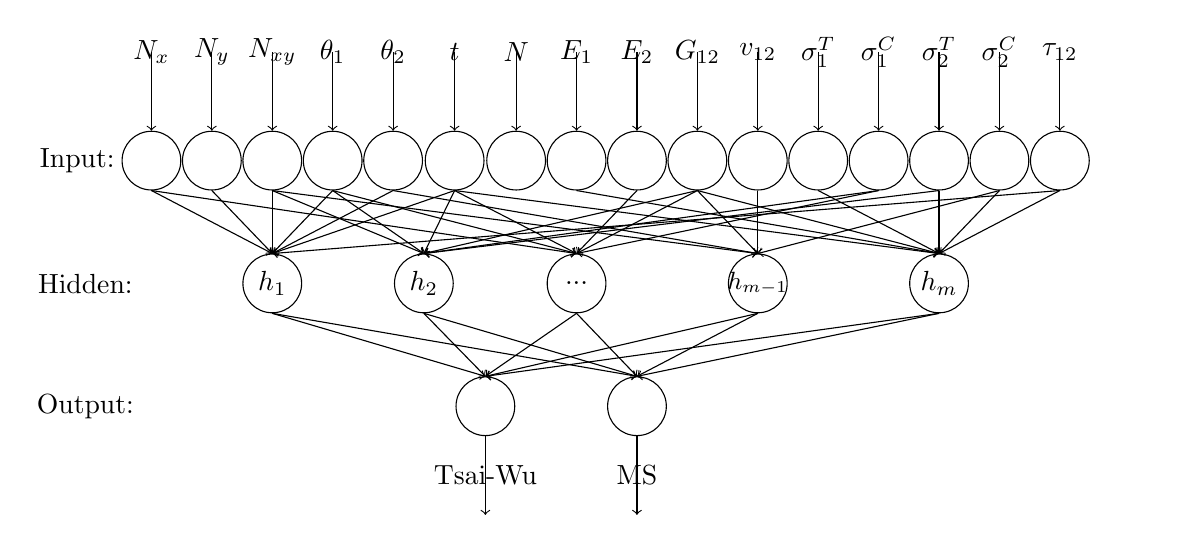
\begin{tikzpicture}
[ p/.style={ draw=none, fill=none, }, remember picture, 
  net/.style={ matrix of nodes, nodes={ draw, circle, inner sep=7.5pt },
  nodes in empty cells,
  column sep=-10.5pt,
  row sep=0.8cm
  }
]
%\draw[help lines] (-3cm,-6cm) grid (6cm,3cm);
\matrix[net] (mat)
{
	  & |[p]| &  & |[p]| &  & |[p]| &  & |[p]| &  & |[p]| &  & |[p]| &  & |[p]| &  & |[p]| &  &
	    |[p]| &  & |[p]| &  & |[p]| &  & |[p]| &  & |[p]| &  & |[p]| &  & |[p]| &  & |[p]|    \\
 |[p]| & |[p]| & |[p]| &  |[p]| &        & |[p]| & |[p]| & |[p]| &|[p]| &       & |[p]| &  |[p]| & |[p]| &
 |[p]| &       & |[p]| &  |[p]| &  |[p]| & |[p]| & |[p]| &       &|[p]| & |[p]| & |[p]| & |[p]|
	   & |[p]| &       &  |[p]| &  |[p]| & |[p]| & |[p]| & |[p]| &|[p]| \\ 
 |[p]| &  |[p]| & |[p]|  &  |[p]| & |[p]|  &  |[p]| &  |[p]| &  |[p]| & |[p]| & |[p]| & |[p]| &       & |[p]|
	   &  |[p]| & |[p]|  &  |[p]| &        &  |[p]| &  |[p]| &  |[p]| & |[p]| & |[p]| & |[p]| & |[p]| &     |[p]|
	   &  |[p]| & |[p]|  &  |[p]| & |[p]|  &  |[p]| &  |[p]| &  |[p]| \\ 
  };
  \draw[<-] (mat-1-1.north) --  ++(0,1) node {$N_x$};
  \draw[<-] (mat-1-3.north) --  ++(0,1) node {$N_y$};
  \draw[<-] (mat-1-5.north) --  ++(0,1) node {$N_{xy}$};
  \draw[<-] (mat-1-7.north) --  ++(0,1) node {$\theta_1$};
  \draw[<-] (mat-1-9.north) --  ++(0,1) node {$\theta_2$};
  \draw[<-] (mat-1-11.north) --  ++(0,1) node {$t$};
  \draw[<-] (mat-1-13.north) --  ++(0,1) node {$N$};
  \draw[<-] (mat-1-15.north) --  ++(0,1) node {$E_1$};
  \draw[<-] (mat-1-17.north) --  ++(0,1) node {$E_2$};
  \draw[<-] (mat-1-19.north) --  ++(0,1) node {$G_{12}$};
  \draw[<-] (mat-1-21.north) --  ++(0,1) node {$v_{12}$};
  \draw[<-] (mat-1-23.north) --  ++(0,1) node {$\sigma_1^T$};
  \draw[<-] (mat-1-25.north) --  ++(0,1) node {$\sigma_1^C$};
  \draw[<-] (mat-1-27.north) --  ++(0,1) node {$\sigma_2^T$};
  \draw[<-] (mat-1-29.north) --  ++(0,1) node {$\sigma_2^C$};
  \draw[<-] (mat-1-31.north) --  ++(0,1) node {$\tau_{12}$};
  \draw[->] (mat-3-12.south) --  ++(0,-1) node[pos=0.5, swap] {Tsai-Wu};
  \draw[->] (mat-3-17.south) --  ++(0,-1) node[pos=0.5, swap] {MS};
  \node at ($(mat-1-1.west)+(-16pt,0)$) {Input: };
  \node at ($(mat-2-2.west)+(-24pt,0)$) {Hidden:};
  \node at ($(mat-3-2.west)+(-24pt,0)$) {Output:};
  \node at (mat-2-5.base) {$h_1$};
  \node at (mat-2-10.base) {$h_2$};
  \node at (mat-2-15.base) {$...$};
  \node at (mat-2-21.base) {\small{$h_{m-1}$}};
  \node at (mat-2-27.base) {$h_{m}$};
 \foreach \a in {1,3,5,7,9,11,31}{
        \draw[->] (mat-1-\a.south) -- (mat-2-5.north);
     }
 \foreach \a in {5,7,11,19,25,27}{
        \draw[->] (mat-1-\a.south) -- (mat-2-10.north);
     }
 \foreach \a in {1,7,11,17,19,25}{
        \draw[->] (mat-1-\a.south) -- (mat-2-15.north);
     }
 \foreach \a in {5,9,19,21,29}{
        \draw[->] (mat-1-\a.south) -- (mat-2-21.north);
     }
 \foreach \a in {11,15,19,23,27,29,31}{
        \draw[->] (mat-1-\a.south) -- (mat-2-27.north);
     }
 \foreach \c in {5,10,15,21,27}{
    \foreach \d in {12,17}{
 		\draw[->] (mat-2-\c.south) -- (mat-3-\d.north);
	}
 }
\end{tikzpicture}
\caption{Neural Network Model}
\end{figure*}

The inputs of the neural network is consist of four parts: in-plane loading
$N_x$, $N_y$, and $N_{xy}$, design parameters of laminate, two distinct fiber
orientation angle $\theta_1$ and $\theta_2$, ply thickness $t$, total number of
plies $N$; five engineering constants of composite materials, $E_1$, $E_2$, ;
five strength parameters of a unidirectional lamina. There are two outputs in
the neural network, safety factors for MS theory and Tsai-Wu theory, respectively.

\begin{figure}
\centering
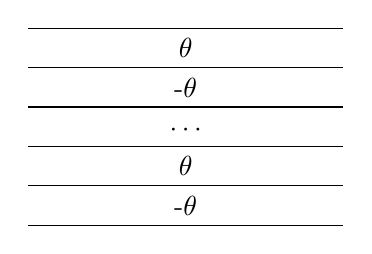
\begin{tikzpicture}
	\draw (0,0) -- (4,0);
	\draw (0,-0.5) -- (4,-0.5) node[midway, above] {$\theta$};
	\draw (0,-1) -- (4,-1) node[midway, above] {\text{-}$\theta$};
	\draw (0,-1.5) -- (4,-1.5) node[midway, above] {$\cdots$};
	\draw (0,-2) -- (4,-2) node[midway, above] {$\theta$};
	\draw (0,-2.5) -- (4,-2.5) node[midway, above] {\text{-}$\theta$};
\end{tikzpicture}
\caption{Model for Angle ply laminate}
\end{figure}


\section{Conclusion}
In this paper, SAGA is proposed to search the optimal lay-up for laminated composite under different
loading. Two situations are considered under the same loading, a set of two distinct angles, and
three distinct angles, SAGA can adjust its convergence speed depending on the difference of
individual's constraint value and constraint threshold.  






\section{The Elsevier article class}

\paragraph{Installation} If the document class \emph{elsarticle} is not available on your computer, you can download and install the system package \emph{texlive-publishers} (Linux) or install the \LaTeX\ package \emph{elsarticle} using the package manager of your \TeX\ installation, which is typically \TeX\ Live or Mik\TeX.

\paragraph{Usage} Once the package is properly installed, you can use the document class \emph{elsarticle} to create a manuscript. Please make sure that your manuscript follows the guidelines in the Guide for Authors of the relevant journal. It is not necessary to typeset your manuscript in exactly the same way as an article, unless you are submitting to a camera-ready copy (CRC) journal.

\paragraph{Functionality} The Elsevier article class is based on the standard article class and supports almost all of the functionality of that class. In addition, it features commands and options to format the
\begin{itemize}
\item document style
\item baselineskip
\item front matter
\item keywords and MSC codes
\item theorems, definitions and proofs
\item lables of enumerations
\item citation style and labeling.
\end{itemize}

\section{Front matter}

The author names and affiliations could be formatted in two ways:
\begin{enumerate}[(1)]
\item Group the authors per affiliation.
\item Use footnotes to indicate the affiliations.
\end{enumerate}
See the front matter of this document for examples. You are recommended to conform your choice to the journal you are submitting to.

\section{Bibliography styles}

There are various bibliography styles available. You can select the style of your choice in the preamble of this document. These styles are Elsevier styles based on standard styles like Harvard and Vancouver. Please use Bib\TeX\ to generate your bibliography and include DOIs whenever available.

Here are two sample references: \cite{Feynman1963118,Dirac1953888}.

\section*{References}

\bibliography{mybibfile}

\end{document}
